\lecture{24}{26. November 2025}{Intro to Turbomachinery Analysis and Pumps}

\section{Fluid Machinery}

\begin{definition}[Fluid Machines]
  A fluid machine is a device that either performs work on or extracts work from a fluid.
\end{definition}

\subsection{Classification of Fluid Machines}
Fluid machines may broadly be classified as either \textit{positive displacement} or \textit{dynamic}.
Dynamic fluid-handling devices that direct the flow using blades or vanes attached to a rotating member are termed \textit{turbomachines}.
In positive-displacement machines, energy transfer is accomplished by volume changes that occur due to movement of the boundary in which the fluid is confined.
This includes piston-cylinder arrangements, gear pumps and lobe pumps.
These will only be reviewed shortly as the emphasis of the course is on dynamic machines.

Furthermore, one can also distinguish types of turbomachines based on the geometry of the flow path.
In \textit{radial-flow} machines, the flow path is (essentially) radial, with significant changes in radius from inlet to outlet.
Such machines are sometimes called \textit{centrifugal} machines.
In \textit{axial-flow} machines, the flow path is nearly parallel to the machine centerline, and the radius of the flow does not vary significantly.
In \textit{mixed-flow} machined the flow-path radius changes moderately.

All work interactions in a turbomachine result from dynamic effects of the rotor on the fluid stream. I.e. the transfer of work between the fluid and the rotating machine will either increase or decrease the speed of flow.
However, in conjunction with this kinetic energy transfer, machines that include external housing also involve either the conversion of pressure energy to kinetic energy or v.v.

\subsubsection{Machines for Doing Work on a Fluid}
Machines that add energy to a fluid by performing work on it are called \textit{pumps}, when the flow is liquid or slurry and \textit{fans}, \textit{blowers}, or \textit{compressors} for gas-handling units depending on pressure rise.

Pumps and compressors consist of a rotating wheel (called an \textit{impeller} or \textit{rotor}, depending on the type of machine) driven by an external power source to increase the kinetic energy of the flow, followed by an element to decelerate the flow, thereby increasing its pressure.
This combination is known as a \textit{stage}.
A single pump or compressor might consist of several stages within a single housing depending on the required pressure rise.

Three typical centrifugal machines are shown on \Cref{fig:f10_1}.
Flow enters each machine nearly axially at small radius through the \textit{eye} of the impeller (a), at radius $r_1$.
Flow is turned and leaves through the impeller discharge at radius $r_2$, where the width is $b_2$.
Ine increase in flow area reduces the fluid velocity and increases the pressure as shown on (b).
(c) shows that the diffuser may have vanes to direct the flow between the impeller discharge and the \textit{volute} (where the fluid is collected).

\begin{figure} [ht]
  \begin{subfigure}{0.3\linewidth}
    \centering
    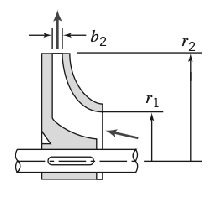
\includegraphics[width=\linewidth]{./figures/f10_1a.png}
    \caption{Centrifugal pump}
  \end{subfigure}
  \begin{subfigure}{0.3\linewidth}
    \centering
    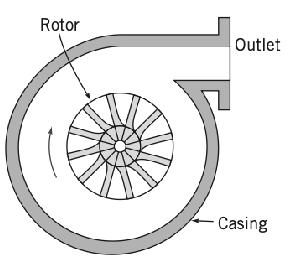
\includegraphics[width=\linewidth]{./figures/f10_1b.png}
    \caption{Centrifugal blower}
  \end{subfigure}
  \begin{subfigure}{0.3\linewidth}
    \centering
    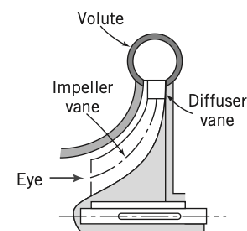
\includegraphics[width=\linewidth]{./figures/f10_1c.png}
    \caption{Centrifugal compressor}
  \end{subfigure}
  \caption{Schematic of typical centrifugal-flow turbomachines.}
  \label{fig:f10_1}
\end{figure}

Typical axial- and mixed-flow turbomachines are shown on \Cref{fig:f10_2}.
(a) shows a typical axial-flow compressor stage.
Here, the rotating element is called a rotor and flow diffusion happens in the stator.
Flow enters nearly  parallel to the rotor axis and maintains nearly the same radius through the stage.
The mixed-flow pump on (b) shows the flow being turned outward moving to larger radius as it passes through the stage.

\begin{figure} [ht]
  \begin{subfigure}{0.48\linewidth}
    \centering
    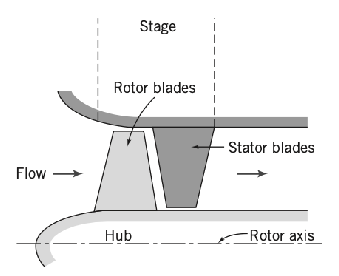
\includegraphics[width=\linewidth]{./figures/f10_2a.png}
    \caption{Axial-flow compressor stage}
  \end{subfigure}
  \begin{subfigure}{0.48\linewidth}
    \centering
    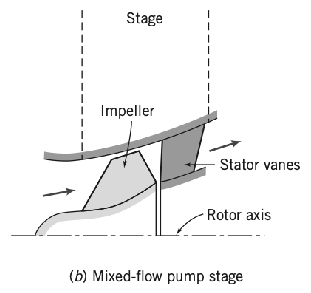
\includegraphics[width=\linewidth]{./figures/f10_2b.png}
    \caption{Mixed-flow pump stage}
  \end{subfigure}
  \caption{Schematic of typical axial- and mixed-flow turbomachines}
  \label{fig:f10_2}
\end{figure}

\subsubsection{Machines for Extracting Work From a Fluid}
Machines that extract energy from a fluid in the form of work are called \textit{turbines}.
In \textit{hydraulic turbines} the working fluid is water, so the flow is incompressible.
In \textit{gas turbines} and \textit{steam turbines}, the density of the working fluid may change significantly.
In a turbine, a stage normally consists of an element to accelerate the flow, converting some of its pressure energy to kinetic energy, followed by a \textit{rotor}, \textit{wheel}, or \textit{runner} that extracts the kinetic energy from the flow via a set of \textit{vanes}, \textit{blades}, or \textit{buckets} mounted on the wheel.

The two most general classifications of turbines are impulse and reaction turbines.
\textit{Impulse turbines} are driven by one or more high-speed free jets.
The classic example of an impulse turbine is the waterwheel.
In more modern forms of impulse turbines, the jet is accelerated in a nozzle external to the turbine wheel.
If friction and gravity are neglected, neither the fluid pressure nor speed relative to the runner changes as the fluid passes over the turbine buckets.
Thus, for an impulse turbine, the fluid acceleration and accompanying pressure drop take place in nozzles external to the blades, and work is extracted as a result of the large momentum change of the fluid.

In \textit{reaction turbines}, part of the pressure change takes place externally and part takes place within the moving blades.
This flow is turned to enter the runner in the proper direction as it passes through nozzles or stationary blades, called \textit{guide vanes} or \textit{wicket gates}.
Additional fluid acceleration relative to the rotor occurs within the moving blades, so both the relative velocity and the pressure of the stream change across the runner.
Because reaction turbines flow full of fluid, they generally can produce more power for a given size than impulse turbines.


\subsection{Turbomachinery Analysis}

\subsubsection{The Angular-Momentum Principle: The Euler Turbomachine Equation} \label{sec:eulerturb}
The angular-momentum principle was applied to control volumes \Cref{sec:angmomprin}, which resulted in\Cref{eq:angmomprin}:
\begin{equation*}
  \Vec{r} \times \Vec{F}_s + \int_{\mathrm{CV}} \Vec{r} \times \Vec{g} \rho \, \mathrm{d}V + \Vec{T}_{\text{shaft}} = \frac{\partial }{\partial t} \int_{\mathrm{CV}} \Vec{r} \times \Vec{V} \rho \, \mathrm{d}V + \int_{\mathrm{CV}} \Vec{r} \times \Vec{V} \rho \Vec{V} \cdot \mathrm{d}\Vec{A}
.\end{equation*}
\Cref{eq:angmomprin} states that the moment of surface forces and body forces, plus the applied torque leads to a change in the angular momentum of the flow.

We will now simplify \Cref{eq:angmomprin} for use in turbomachinery analysis.
First it is convenient to choose a fixed control volume enclosing the rotor to evaluate shaft torque.
Because we are looking at control volumes for which we expect large shaft torques, as a first approximation torques due to surface forces may be ignored.
This means we are neglecting friction and torque generated by pressure changes.
The body force may be neglected by symmetry.
Then for steady flow, \Cref{eq:angmomprin}, reduces to:
\begin{equation} \label{eq:angmomprinturb}
  \Vec{T}_{\text{shaft}} = \int_{\mathrm{CV}} \Vec{r} \times \Vec{V} \rho \Vec{V} \cdot \mathrm{d}\Vec{A}
.\end{equation}
This states, that for a turbomachine with work \textit{input}, the torque \textit{required} causes a change in the angular momentum of the fluid.
For a turbomachine with work \textit{output}, the torque \textit{produced} is due to the change in angular momentum of the fluid.

As depicted on \Cref{fig:f10_6}, we select a fixed control volume enclosing a generalized turbomachine rotor.
The idealized velocity components are shown in the figure.
The fluid enters the rotor at radial location $r_1$ with uniform absolute velocity, $\Vec{V}_1$; the fluid leaves the rotor at radial location $r_2$ with uniform absolute velocity $\Vec{V}_2$.
\begin{figure} [ht]
  \centering
  
\includegraphics[width=0.5\linewidth]{./figures/f10_6.png}
  \caption{Finite control volume and absolute velocity components for analysis of angular momentum.}
  \label{fig:f10_6}
\end{figure}
For \textit{uniform flow} into the rotor at Section 10.2 and out of the rotor at Section 10.2, \Cref{eq:angmomprinturb} becomes:
\begin{equation*}
  T_{\text{shaft}} \hat{k} = \left( r_2 V_{t_2} - r_1 V_{t_1} \right) \dot{m} \hat{k} 
.\end{equation*}
For the product $\Vec{r} \times \Vec{V}$, the position vector is purely radial and only the tangential velocity component $V_t$ counts.
In scalar form:
\begin{equation*}
  T_{\text{shaft}} = \left( r_2 V_{t_2} - r_1 V_{t_1} \right) \dot{m}
.\end{equation*}
The assumptions behind this equation are \textit{steady}, \textit{frictionless flow}, \textit{uniform flow} at inlet, and exit and \textit{negligible pressure effects}.

The rate of work $\dot{W}_m$ done on a turbomachine rotor is given by the dot product of rotor angular velocity $\Vec{\omega}$ and applied torque $\Vec{T}_{\text{shaft}}$.
Using the result from before, we obtain
\begin{equation*}
  \dot{W}_m = \Vec{\omega} \cdot \Vec{T}_{\text{shaft}} = \omega \hat{k} \cdot T_{\text{shaft}} \hat{k} = \omega \hat{k} \cdot \left( r_2 V_{t_2} - r_1 V_{t_1} \right) \dot{m} \hat{k}
\end{equation*}
or
\begin{equation*}
  \dot{W}_m = \omega T_{\text{shaft}} = \omega \left( r_2 V_{t_2} - r_1 V_{t_1} \right) \dot{m}
.\end{equation*}

We introduce $U = r \omega$, where $U $ is the tangential speed of the rotor at radius $r$, we have
\begin{equation} \label{eq:102b}
  \dot{W}_m = \left( U_2 V_{t_2} - U_1 V_{t_1} \right)\dot{m}
.\end{equation}
Dividing \Cref{eq:102b} by $\dot{m}g$ we obtain a quantity with dimensions of length, which may be viewed as the theoretical head added to the flow:
\begin{equation*}
  H = \frac{\dot{W}_m}{\dot{m} g} = \frac{1}{g} \left( U_2 V_{t_2} - U_1 V_{t_1} \right)
.\end{equation*}

\subsubsection{Velocity Diagrams}
The equations we derived in \Cref{sec:eulerturb} suggest the importance of clearly defining the velocity components of the fluid and rotor at the inlet and outlet sections.
For this purpose, it is useful to develop \textit{velocity diagrams} for the inlet and outlet flows. \Cref{fig:f10_7} shows the velocity diagrams and introduced the notation for blade and flow angles.
The important notation to remember is that the variable $V$ is typically used to indicate absolute velocity, while the variable $W$ is used to indicate flow velocity relative to the rotating blade.

\begin{figure} [ht]
  \begin{subfigure}{0.4\linewidth}
    \centering
    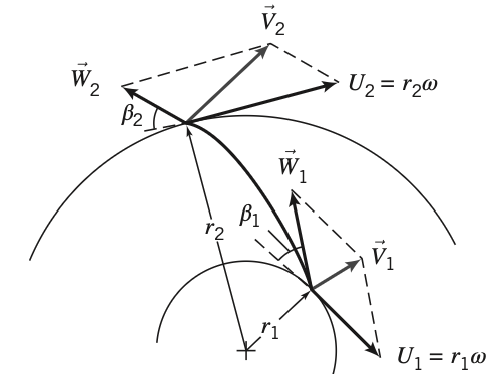
\includegraphics[width=\linewidth]{./figures/f10_7a.png}
    \caption{Absolute velocities as som of velocity relative to blade and rotor velocity}
  \end{subfigure}
  \begin{subfigure}{0.28\linewidth}
    \centering
    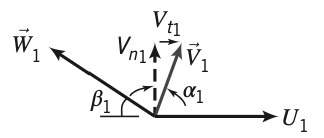
\includegraphics[width=\linewidth]{./figures/f10_7b.png}
    \caption{Velocity components at inlet}
  \end{subfigure}
  \begin{subfigure}{0.28\linewidth}
    \centering
    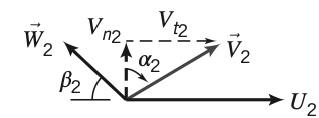
\includegraphics[width=\linewidth]{./figures/f10_7c.png}
    \caption{Velocity components at outlet}
  \end{subfigure}
  \caption{Geometry and notation used to develop velocity diagrams for radial-flow machines.}
  \label{fig:f10_7}
\end{figure}

Machines are designed in a manner, such that at \textit{design condition} the fluid moves smoothly through the blades.
In the idealized situation at the \textit{design speed}, sometimes called \textit{shockless entry}, flow relative to the rotor is assumed to enter and leave tangent to the blade profile at each section.
At speeds other than the design speed, the fluid may impact the blades at inlet, exit at an angle relative to the blade, or may have significant flow separation, leading to inefficiency. \Cref{fig:f10_7} is representative of a typical radial flow machine.
We assume that the fluid is moving without major flow disturbances through the machine, as shown in \Cref{fig:f10_7}a, with blade inlet and exit angles $\beta_1$ and $\beta_2$, respectively, relative to the circumferential direction.
In general $\beta_1$ and $\beta_2$ may be any angle from \ang{0} to \ang{180}.

The runner speed at the inlet is $U_1 = r_1 \omega$, and therefore it is specified by the impeller geometry and the operating speed.
The absolute fluid velocity is the vector sum of the impeller velocity and the flow velocity relative to the blade.
The absolute inlet velocity may be determined graphically, as shown in \Cref{fig:f10_7}b.
The angle of the absolute fluid velocity $\alpha_1$ is measured from the direction normal to the flow area.
For a given machine, $\alpha_1$ and $\alpha_2$ will vary with flow rate $Q$ and rotor speed $\omega$.
The tangential component of the absolute velocity $V_{t_1}$ and the component normal to the flow area $V_{n_1}$ are also shown on \Cref{fig:f10_7}b. 
At each section the normal component of the absolute velocity $V_n$ and the normal component relative to the velocity of the blade $W_n$ are equal because the blade has no normal velocity.

The velocity diagram is constructed similarly at the outlet section.
The runner speed at the outlet is $U_2 = r_2 \omega$, which again is known from the geometry and operating speed of the turbomachine.
The relative flow is assumed to leave the impeller tangent to the blades as shown on \Cref{fig:f10_7}c.

For a centrifugal pump or reaction turbine, the velocity relative to the blade generally changes in magnitude from the inlet to outlet.
The continuity equation must be applied to determine the normal component of velocity at each section.
The normal component together with the flow outlet blade angle is sufficient to establish the velocity relative to the blade impeller outlet for a radial-flow machine.
The velocity diagram is completed by the vector addition of the velocity relative to the blade and the wheel velocity as depicted on \Cref{fig:f10_7}c.

Due to the idealized assumptions the analytical result will often represent a sort of upper limit of the performance of actual machines.

\subsubsection{Performance--Hydraulic Power}
The torque and power predicted by applying the angular momentum equation to a turbomachine rotor are idealized values.
In practice, rotor power and the rate of change of fluid energy are not equal.
Losses are caused by viscous effects, non-uniform flow, mismatched flow direction and blade angle, and inefficiencies in the diffuser. 
Energy dissipation occurs in seals and bearings and in fluid friction between the rotor and housing of the machine (so-called \textit{windage} losses).
Because of these losses, in a pump, the actual power delivered to the fluid is less than predicted by the angular-momentum equation.
In the case of a turbine, the actual power delivered to the shaft is less than the power given up by the fluid stream.

We define the power, head and efficiency of a turbomachine based on whether the machine does work on the fluid or extracts work from the fluid.
For a pump, the \textit{hydraulic power} is given by the rate of mechanical energy input to the fluid,
\begin{equation*}
  \dot{W}_h = \rho Q g H_p
\end{equation*}
where
\begin{equation*}
  H_p = \left( \frac{p}{\rho g} + \frac{\overline{V}^2}{2g} + z \right)_{\text{discharge}} - \left( \frac{p}{\rho g} + \frac{\overline{V}^2}{2g} + z \right)_{\text{suction}}
.\end{equation*}

The mechanical input power needed to drive the pump is greater then that to produce the head rise due to inefficiencies.
We define the \textit{pump efficiency as}
\begin{equation*}
  \eta_p \equiv \frac{\dot{W}_h}{\dot{W}_m} = \frac{\rho Q g H_p}{\omega T}
.\end{equation*}

For a hydraulic turbine, the \textit{hydraulic power} is defined as the rate of mechanical energy removal from the flowing fluid stream,
\begin{equation*}
  \dot{W}_h = \rho Q g H_t
\end{equation*}
where
\begin{equation*}
  H_p = \left( \frac{p}{\rho g} + \frac{\overline{V}^2}{2g} + z \right)_{\text{inlet}} - \left( \frac{p}{\rho g} + \frac{\overline{V}^2}{2g} + z \right)_{\text{outlet}}
.\end{equation*}

The mechanical power output obtained form the turbine is related to the hydraulic power by defining \textit{turbine efficiency} as
\begin{equation*}
  \eta_t \equiv \frac{\dot{W}_m}{\dot{W}_h} = \frac{\omega T}{\rho Q g H_t}
.\end{equation*}

Therefore, to obtain maximum power from a hydraulic turbine, one must minimize the mechanical energy in the flow leaving the turbine.
This is accomplished by making the outlet pressure, flow speed, and elevation as small as practical.

\subsection{Pumps, Fans, and Blowers}

\subsubsection{Application of Euler Turbomachine Equation to Centrifugal Pumps}
With $V_{t_1} = 0$, the increase in head is given by
\begin{equation*}
  H = \frac{U_2 V_{t_2}}{g}
.\end{equation*}
From the exit velocity diagram of \Cref{fig:f10_7}c,
\begin{equation*}
  V_{t_2} = U_2 - W_2 \cos\beta_2 = U_2 - \frac{V_{n_2}}{\sin \beta_2} \cos \beta_2 = U_2 - V_{n_2} \cot \beta_2 
.\end{equation*}
Then
\begin{equation*}
  H = \frac{U_2^2 - U_2 V_{n_2} \cot \beta_2}{g}
.\end{equation*}
For an impeller of width $w$, the volume flow rate is
\begin{equation} \label{eq:volflow}
  Q = \pi D_2 w V_{n_2}
.\end{equation}
To express the increase in head in terms of volume flow rate, we substitute for $V_{n_2}$ in terms of $Q$ from \Cref{eq:volflow}. Thus
\begin{equation} \label{eq:headlosslin}
  H = \frac{U_2^2}{g} - \frac{U_2 \cot \beta_2}{\pi D_2 wg} Q
.\end{equation}
This is an equation of the form
\begin{equation*}
  H = C_1 - C_2 G
\end{equation*}
where constants $C_1$ and $C_2$ are functions of \textit{machine geometry} and \textit{speed}.

Therefore, \Cref{eq:headlosslin} predicts a linear variation of head $H$ with volume flow rate $Q$.
Constant $C_1 = U_2^2 / g$ represents the ideal head developed by the pump for zero flow rate and is called the \textit{shutoff head}.
The linear relation is an idealized model and actual devices may only approximate linear variation.

For radial outlet vanes, $\beta_2 = \ang{90}  $ and $C_2 = 0$.
The tangential component of the absolute velocity at the outlet is equal to the wheel speed and is independent of flow rate.
From \Cref{eq:headlosslin} the ideal head is independent of flow rate.
The characteristic $H-Q$ curve is shown on \Cref{fig:f10_12}.

\begin{figure} [ht]
  \centering
  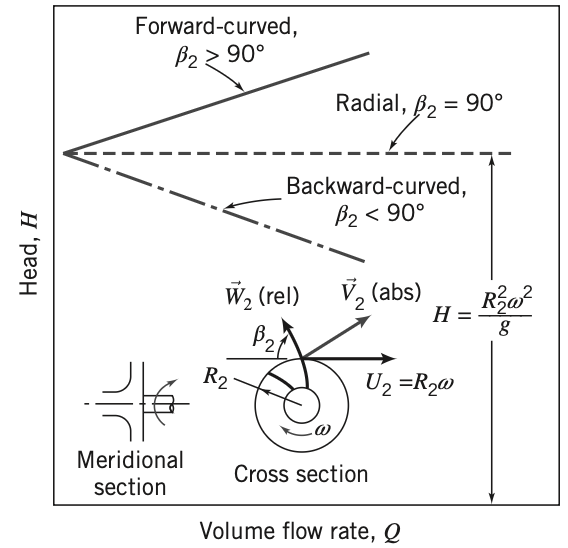
\includegraphics[width=0.8\linewidth]{./figures/f10_12.png}
  \caption{Idealized relationship between head and volume flow rate for centrifugal pump with forward-curved, radial, and backward-curved impeller blades.}
  \label{fig:f10_12}
\end{figure}

If the vanes are forward curved, then $\beta_2 > \ang{90} $ and $C_2 < 0$.
The tangential component of the absolute fluid velocity at the outlet is greater than the wheel speed, and it increases as the flow rate increases.


\subsubsection{Performance Characteristics}
To specify fluid machines for flow systems, the designer must know the pressure rise (or head), torque, power requirement, and efficiency of a machine.
For a given machine, each of these characteristics is a function of flow rate and for similar machines depend on size and operating speed.

On \Cref{fig:f10_13} idealized and actual head-flow curves are plotted.
This shows that the head at any flow rate in the real machine may be significantly lower than predicted by the idealized analysis.
Some of the causes are that at very low flow rate, some fluid recirculates in the impeller, friction loss and leakage loss both increase with flow rate, and ``shock loss'' results from a mismatch between the direction of the relative velocity and the tangent to the impeller blade at the inlet.

The curve shown on \Cref{fig:f10_13} is measured at constant (design) speed with a single impeller diameter.
It is common practice to vary pump capacity by changing the impeller size in a given casing.

\begin{figure} [ht]
  \centering
  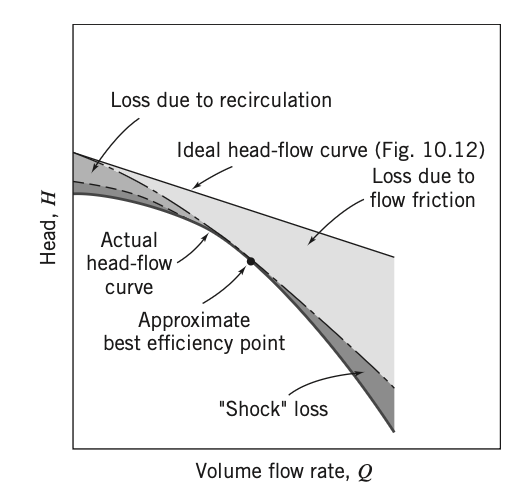
\includegraphics[width=0.8\linewidth]{./figures/f10_13.png}
  \caption{Comparison of ideal and actual head-flow curves for a centrifugal pump with backward-curved impeller blades}
  \label{fig:f10_13}
\end{figure}

\subsubsection{Pump Selection in Fluid Systems}
\begin{definition}[Fluid System]
 We define a \textit{fluid system} as the combination of a fluid machine and a network of pipes or channels that convey fluid.
\end{definition}

A typical pump produces a smaller head at higher pressure as the flow rate is increased.
In contrast, the head required to maintain flow in a pipe system increases with the flow rate due to increased losses.
Therefore a pump system will operate at the flow rate at which the pump head rise and required system head match.
This is termed the operating point.

The required head for a system with no static lifts starts at zero flow and head and increases with flow.
In this case, the total head required is the sum of major and minor losses,
\begin{equation*}
  h_{l_t} = \sum h_l + \sum h_m  = \sum f \frac{L}{D} \frac{\overline{V}^2}{2} + \sum K \frac{\overline{V}^2}{2}
.\end{equation*}
For turbulent flow, the friction factors are nearly constant with flow and the minor loss coefficients $K$ are also constant.
Hence $h_{l_t} \sim \overline{V}^2 \sim Q^2$ so that the system curve is approximately parabolic.
This means that the system curve with pure friction becomes steeper as flow rate increases.

Whether the resulting system curve is \textit{steep} or \textit{flat} depends on the relative importance of friction and gravity.
Friction drop may be relatively unimportant in the water supply to a high-rise building and gravity lift may be negligible in an air-handling system for a one-story building.
